\documentclass{beamer}
\beamertemplatenavigationsymbolsempty
\usecolortheme{beaver}
\setbeamertemplate{blocks}[rounded=true, shadow=true]
\setbeamertemplate{footline}[page number]
%
\usepackage[utf8]{inputenc}
\usepackage[english,russian]{babel}
\usepackage{amssymb,amsfonts,amsmath,mathtext}
\usepackage{subfig}
\usepackage[all]{xy} % xy package for diagrams
\usepackage{array}
\usepackage{multicol}% many columns in slide
\usepackage{hyperref}% urls
\usepackage{hhline}%tables
% Your figures are here:
\graphicspath{ {fig/} {../paper/figures} }

%----------------------------------------------------------------------------------------------------------
\title[\hbox to 56mm{Восстанвление прогноза}]{Восстановление прогноза, сделанного в метрическом вероятностном пространстве, в исходное пространство (временных рядов)}
\author[М. М. Дивильковский]{Максим Михайлович Дивильковский}
\institute{Московский физико-технический институт}
\date{\footnotesize
	\par\smallskip\emph{Курс:} Автоматизация научных исследований\par (практика, В.\,В.~Стрижов)/Группа 125
	\par\smallskip\emph{Эксперт:} В. В. Стрижов
	\par\smallskip\emph{Консультант:} К. Д. Яковлев
	\par\bigskip\small 2024}
%----------------------------------------------------------------------------------------------------------
\begin{document}
	%----------------------------------------------------------------------------------------------------------
	\begin{frame}
		\thispagestyle{empty}
		\maketitle
	\end{frame}
	%-----------------------------------------------------------------------------------------------------
	%-----------------------------------------------------------------------------------------------------
	\begin{frame}{Доклад с одним слайдом}
		
		\begin{columns}[c]
			\column{0.5\textwidth}
			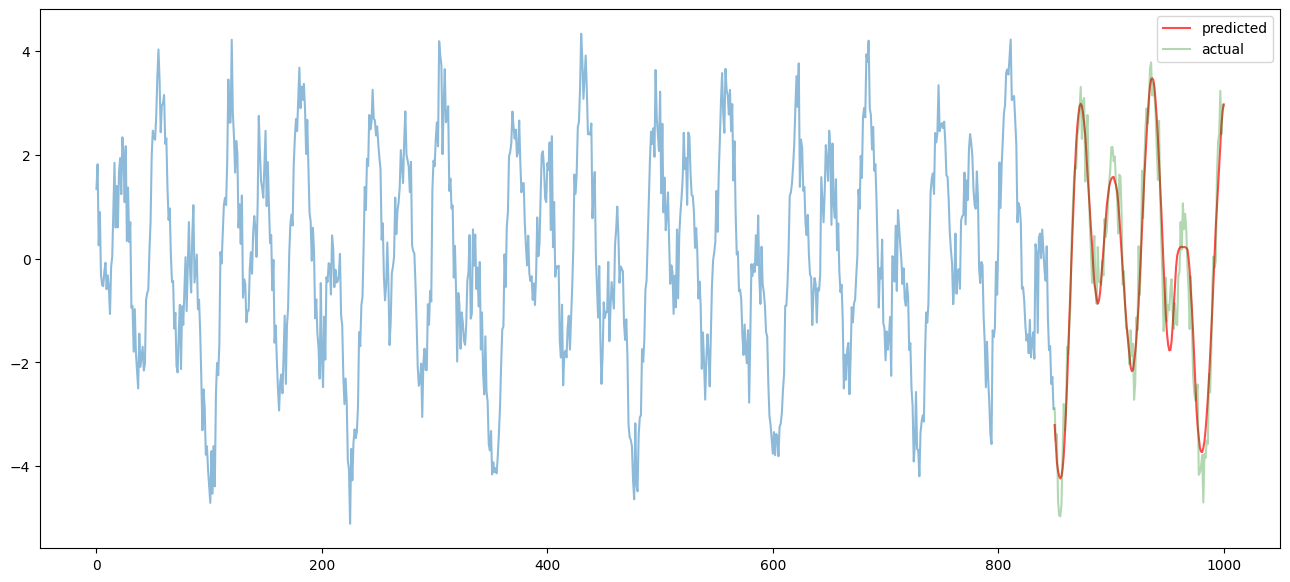
\includegraphics[width=1.0\textwidth]{LSTM-prediction}
			Предсказание методом LSTM
			\column{0.5\textwidth}
			\includegraphics[width=1.0\textwidth]{Several-Series}
			Ряды высокой попарной корреляции
		\end{columns}
		
		\bigskip
		\begin{itemize}
			\item $X$~--- линейное пространство временных рядов. $X \cong \mathbb{R}^{T}$
			\item $\rho(x, y), x, y \in X$~--- расстояния в $X$
			\item $X \rightarrow \Sigma_T$~--- матрица попарных расстояний
			\item $\Sigma_T \rightarrow \Sigma_{T+1}$~--- прогноз в следующий момент времени
			\item $\Sigma_{T+1} \rightarrow \hat{X}$~--- {\color{red}восстановление прогноза}
		
		\end{itemize}
	\end{frame}
	
	
\end{document} 